% -*- mode: noweb; noweb-default-code-mode: R-mode; -*-


%\SweaveOpts{ eps=FALSE, pdf=FALSE, png=TRUE }

\graphicspath{ {analysis/} }

\chapter{Analysis}
\label{cha:analysis}


% latex table generated in R 2.11.1 by xtable 1.5-6 package
% Mon Dec  6 14:40:52 2010
\begin{table}[ht]
\begin{center}
\begin{tabular}{rrrrrrrrrr}
  \hline
 & crop & open & barren & forest & shrub & urban & water & wetland & mosaic \\ 
  \hline
As00 & 369.6 & 545.8 & 28.9 & 353.6 & 341.8 & 29.8 & 75.0 & 11.0 & 237.0 \\ 
  As05 & 379.2 & 516.3 & 32.9 & 344.5 & 359.1 & 27.3 & 73.4 & 26.1 & 232.8 \\ 
  ag & 446.5 & 557.1 &  &  &  &  &  &  &  \\ 
  agc & 450.1 & 558.3 & 25.3 & 450.3 & 368.0 & 35.1 & 74.5 & 30.9 &  \\ 
  nlcd & 310.8 & 429.6 & 24.5 & 513.2 & 420.1 & 102.8 & 96.5 & 95.0 &  \\ 
   \hline
\end{tabular}
\caption{Total Acreages by Map and Cover}
\label{tab:total}
\end{center}
\end{table}
The MLCT indicates 379.2Ma (153.4Mha) of
cropland in the cUSA in 2001. Assuming that 50\% of the
cropland/natural vegetation mosaic is additional cropland area gives
an additional 116.4Ma (47.1Mha)
of agricultural land. This gives a total area of 
495.6Ma (200.6Mha)
of total area directly associated with
agricultural activity according to the IGBP classification used in the
MLCT.

Aglands2000 indicates roughly 446.5Ma (180.7Mha) 
of cropland.

Pasture indicated by Aglands2000 appears to be a broader
classification than that of the NLCD's pasture class because much of
the grazing land east of the Mississippi river counted in the
Aglands2000 pasture map is absent in the NLCD pasture class.

Due to its greater resolution (30m) the NLCD is better suited at
discerning developed areas in rural landscapes ranging from rural
roads to farmsteads to small communities that do not show up in the
MLCT data. There is a total area of roughly 74 Ma (30 Mha) of
development remaining after subtracting the MLCT urban class from all
developed classes in the NLCD where the NLCD shows greater development
after they have both been aggregated to the 5-arcmin grid. Applying
this area as an offset to the cropland area in Aglands2000 brings us
closer to the expected acreage under cultivation in 2001, although
this assumes that all of that development intersects with MLCT
cropland area.


% latex table generated in R 2.11.1 by xtable 1.5-6 package
% Mon Dec  6 14:44:54 2010
\begin{table}[ht]
\begin{center}
\begin{tabular}{rrrrr}
  \hline
 & rmse\_frac & bias\_frac & rmse\_acres & bias\_acres \\ 
  \hline
barren & 0.05 & 2.68E-04 & 902 & 7 \\ 
  crop & 0.15 & 6.94E-02 & 2515 & 1142 \\ 
  forest & 0.20 & -2.82E-02 & 3249 & -516 \\ 
  open & 0.32 & 6.13E-02 & 5418 & 1056 \\ 
  shrub & 0.33 & -2.65E-02 & 5572 & -427 \\ 
  urban & 0.06 & -3.34E-02 & 973 & -555 \\ 
  water & 0.04 & -1.11E-02 & 580 & -181 \\ 
  wetland & 0.10 & -3.16E-02 & 1608 & -526 \\ 
   \hline
\end{tabular}
\caption{Errors and Biases of Aglands Complete relative to NLCD}
\label{tab:ebagc}
\end{center}
\end{table}% latex table generated in R 2.11.1 by xtable 1.5-6 package
% Mon Dec  6 14:44:54 2010
\begin{table}[ht]
\begin{center}
\begin{tabular}{rrrrr}
  \hline
 & rmse\_frac & bias\_frac & rmse\_acres & bias\_acres \\ 
  \hline
barren & 0.07 & 1.95E-03 & 1140 & 36 \\ 
  crop & 0.19 & 3.18E-02 & 2945 & 482 \\ 
  forest & 0.20 & -7.77E-02 & 3380 & -1309 \\ 
  open & 0.33 & 5.84E-02 & 5428 & 953 \\ 
  shrub & 0.29 & -4.34E-02 & 4783 & -642 \\ 
  urban & 0.06 & -3.62E-02 & 988 & -598 \\ 
  water & 0.03 & -1.09E-02 & 504 & -177 \\ 
  wetland & 0.10 & -4.15E-02 & 1759 & -689 \\ 
   \hline
\end{tabular}
\caption{Errors and Biases of MLCT, $A_s = 0.0$ relative to NLCD}
\label{tab:ebmlct00}
\end{center}
\end{table}% latex table generated in R 2.11.1 by xtable 1.5-6 package
% Mon Dec  6 14:44:54 2010
\begin{table}[ht]
\begin{center}
\begin{tabular}{rrrrr}
  \hline
 & rmse\_frac & bias\_frac & rmse\_acres & bias\_acres \\ 
  \hline
barren & 0.06 & 3.89E-03 & 1092 & 69 \\ 
  crop & 0.17 & 3.63E-02 & 2690 & 560 \\ 
  forest & 0.20 & -8.21E-02 & 3362 & -1383 \\ 
  open & 0.30 & 4.35E-02 & 4891 & 711 \\ 
  shrub & 0.27 & -3.43E-02 & 4410 & -500 \\ 
  urban & 0.06 & -3.74E-02 & 1027 & -619 \\ 
  water & 0.03 & -1.17E-02 & 529 & -190 \\ 
  wetland & 0.10 & -3.42E-02 & 1595 & -565 \\ 
   \hline
\end{tabular}
\caption{Errors and Biases of MLCT, $A_s = 0.5$ relative to NLCD}
\label{tab:ebmlct05}
\end{center}
\end{table}

\begin{figure} 
\begin{center} 
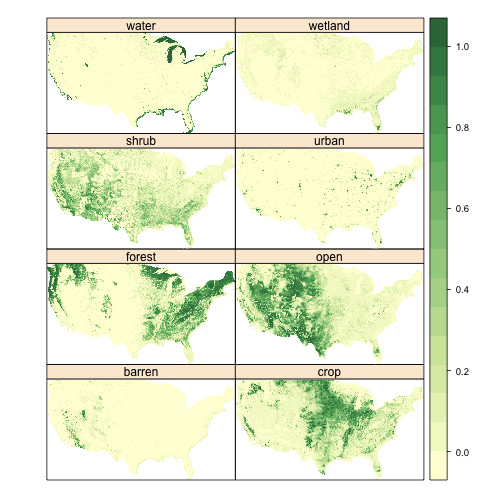
\includegraphics{fig_agc}
\end{center} 
\caption{Aglands Complete cover maps} 
\label{fig:agc} 
\end{figure} 

\begin{figure} 
\begin{center} 
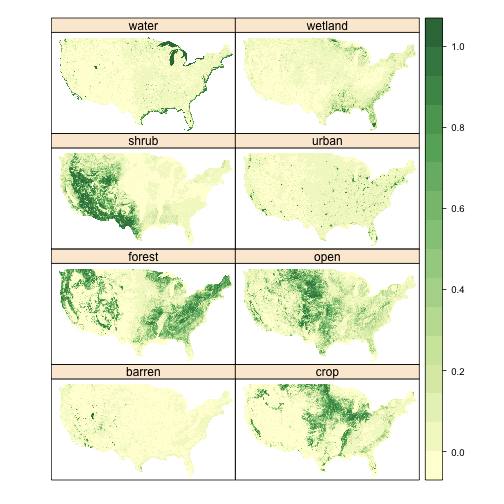
\includegraphics{fig_nlcd}
\end{center} 
\caption{NLCD cover maps} 
\label{fig:nlcd} 
\end{figure} 

\begin{figure} 
\begin{center} 
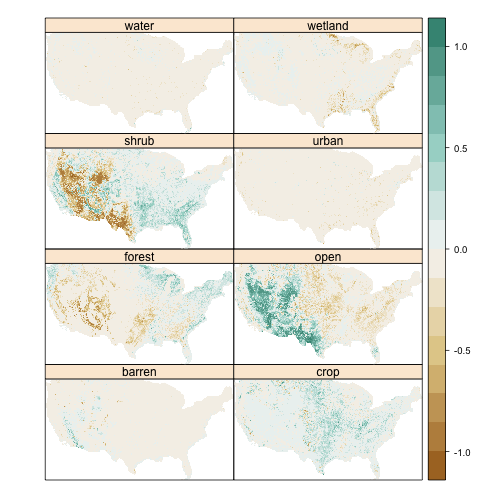
\includegraphics{fig_diff}
\end{center} 
\caption{Difference maps, Aglands Complete minus NLCD} 
\label{fig:diff} 
\end{figure} 

\begin{figure} 
\begin{center} 
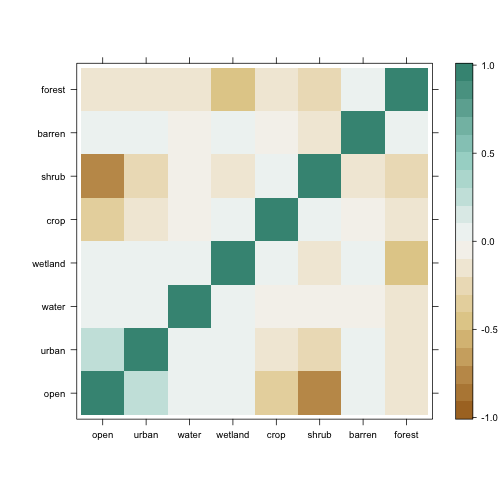
\includegraphics{fig_cordiff}
\end{center} 
\caption{Correlations across cover type in difference maps} 
\label{fig:cordiff} 
\end{figure} 

The elements of the matrix have been reordered according to the
clustering forumla given in \citet[sec. 6.2.3]{Sarkar2008} in order to
achieve a degree of visual clustering among the correlation vectors.

%%% Local Variables: 
%%% mode: latex
%%% TeX-master: "thesis"
%%% End: 
